\documentclass[11pt]{article}
\twocolumn
\setlength{\columnsep}{30pt}
\usepackage{graphicx} % Required for inserting images
\usepackage[a4paper, margin=1.5cm]{geometry}
\usepackage{times}
\usepackage{polski}
\usepackage{enumitem}
\renewcommand{\thesection}{\Roman{section}} 
\renewcommand{\thesubsection}{\Alph{subsection}}
\usepackage{hyperref} % Required for hyperlinks

\usepackage[backend=biber, style=numeric]{biblatex}
\addbibresource{bibliografia.bib}

\newcommand{\mycomment}[1]{}

\title{{\Huge Analiza posiadania piłki drużyn piłkarskich w zależności od różnych czynników meczowych}}
\author{Dominik Patrzek\\
WIT IST\\
266585@student.pwr.edu.pl\\
 MSiD 17:05 TP}
\date{15 czerwca 2023}


\begin{document}

\maketitle

\section{Wstęp}
Wybranym do analizy zagadnieniem jest posiadanie piłki w zależności od różnych czynników. Drużyny mające dużo posiadania grają atrakcyjny futbol, przyjemny dla oka kibica. Jakie więc kryteria należy spełniać, aby zainteresować więcej ludzi swoimi meczami? W badaniu posiadanie piłki zostanie zbadane w zestawieniu z parametrami takimi jak:
\begin{itemize}[itemsep=1pt, topsep=1pt]
  \item liczba strzałów na bramkę
  \item liczba oczekiwanych goli
  \item liczba fauli drużyny przeciwnej
  \item poziom drużyny
  \item liczba rzutów rożnych
  \item pogoda
  \newline
\end{itemize}
Ponadto stworzony zostanie model, który estymuje posiadanie piłki drużyny na podstawie wybranych czynników.

\section{Zbiór danych i jego przetwarzanie}
\subsection{Zbiór danych}

Zbiór danych został pozyskany ze źródła footystats\cite{footystats}. Przedstawia on wiele statystyk dotyczących wszystkich meczów Premier League z sezonu 2018/19 zakończonego tryumfem drużyny Manchesteru City. Posiadanie piłki jest wartością procentową, reszta statystyk to liczby całkowite i rzeczywiste dodatnie. Ponadto użyta została Weather API ze źródła visualcrossing\cite{weather}, zostały do niej wysyłane zapytania, aby otrzymać dane pogodowe w miejscu danego wydarzenia.


\subsection{Przetwarzanie wstępne}
Ze zbioru danych zostału usunięte dane, które nie będą brały udziału w badaniu. Pod uwagę będą brane statystyki posiadania piłki itd. w kontekście drużyny gospodarza meczu.

\subsection{Analiza eksploracyjna}


Spójrzmy na cechy zbioru posiadania piłki
\mycomment{
\begin{center}
    \begin{tabular}{| c | c |}
    \hline
    Wartość min. & 18\% \\ \hline
    Wartość max. & 80\%  \\ \hline
    Mediana & 51.0\%  \\ \hline
    Odchyl. standardowe & 13.84\%  \\ \hline
    Najczęściej wyst. wartość & 62\% \\ \hline
    Najrzadziej wyst. wartość & 79\% \\ \hline
    \end{tabular}
\end{center}
}

\begin{table}[htb]
\centering
\begin{tabular}{| c | c |}
\hline
Wartość min. & 18\% \\ \hline
Wartość max. & 80\% \\ \hline
Mediana & 51.0\% \\ \hline
Odchyl. standardowe & 13.84\% \\ \hline
Najczęściej wyst. wartość & 62\% \\ \hline
Najrzadziej wyst. wartość & 79\% \\ \hline
\end{tabular}
\caption{Cechy posiadania piłki}
\label{tab:moja-tabela}
\end{table}

%\clearpage
Odchylenie standardowe, które otrzymano może być uważane za umiarkowane. Oznaczające pewną zmienność, ale nie jest to ekstremalnie duże odchylenie.

\begin{figure}[hbt]
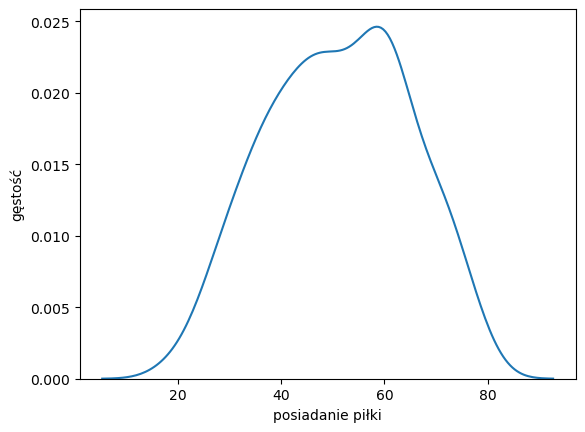
\includegraphics[scale=0.30]{distribution.png}
\caption{Rozkład posiadania piłki}
\end{figure}

Po przetwarzaniu wstępnym zbiór zawiera dane 380 meczów scharakteryzowanych 13 cechami. 

W mapie korelacji zmiennych można zauważyć wysoką zależność między posiadaniem piłki, a wskaźnikiem oczekiwanych goli i poziomem drużyny.

\begin{figure}[hbt]
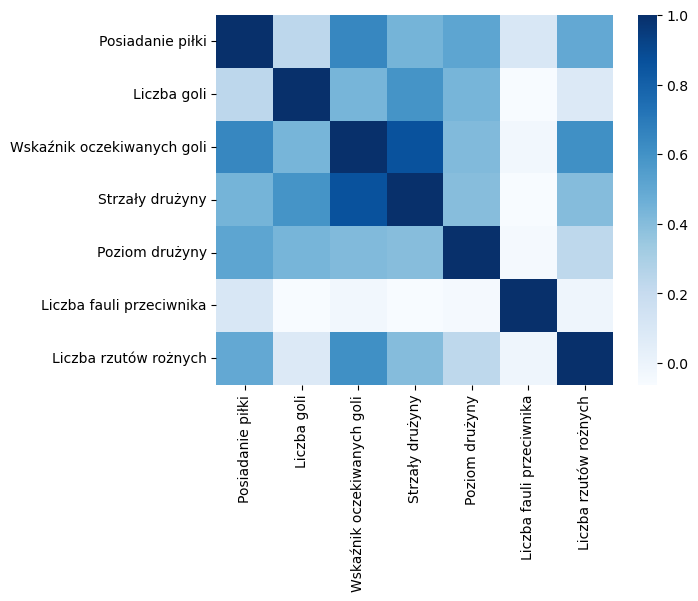
\includegraphics[scale=0.35]{heatmap.png}
\caption{Mapa korelacji zmiennych}
\end{figure}


\section{Eksperymenty}
%\renewcommand{\thesection}{\Roman{section}}
\renewcommand{\thesubsection}{\arabic{subsection}}
\subsection{Opis eksperymentów}

\begin{enumerate}[label=\alph*)]
  \item Eksperyment 1 - dopasowanie modelu regresji liniowej oraz wielomianu n-tego stopnia do danych dotyczących liczby strzałów oddanych przez drużynę w meczu.
  \item Eksperyment 2 - dopasowanie modelu regresji liniowej oraz wielomianu n-tego stopnia do danych dotyczących osiągniętego współczynnika goli oczekiwanych przez drużynę. 
  \item Eksperyment 3 - dopasowanie modelu regresji liniowej oraz wielomianu n-tego stopnia do danych dotyczących liczby fauli popełnionych przez drużynę przeciwną.
  \item Eksperyment 4 - dopasowanie modelu regresji liniowej oraz wielomianu n-tego stopnia do danych dotyczących poziomu drużyny grającej mecz (mierzona średnią punktowania drużyny na mecz). 
  \item Eksperyment 5 - dopasowanie modelu regresji liniowej oraz wielomianu n-tego stopnia do danych dotyczących liczby rzutów rożnych wykonanych przez drużynę.
  \item Eksperyment 6 - dopasowanie modelu regresji liniowej oraz wielomianu n-tego stopnia do danych dotyczących pogody w trakcie meczów Manchesteru City - najlepszej drużyny sezonu.
\end{enumerate}
\newpage
\subsection{Właściwe eksperymenty}

\begin{enumerate}[label=\alph*)]
  \item Eksperyment 1 \newline

    \begin{figure}[hbt]
    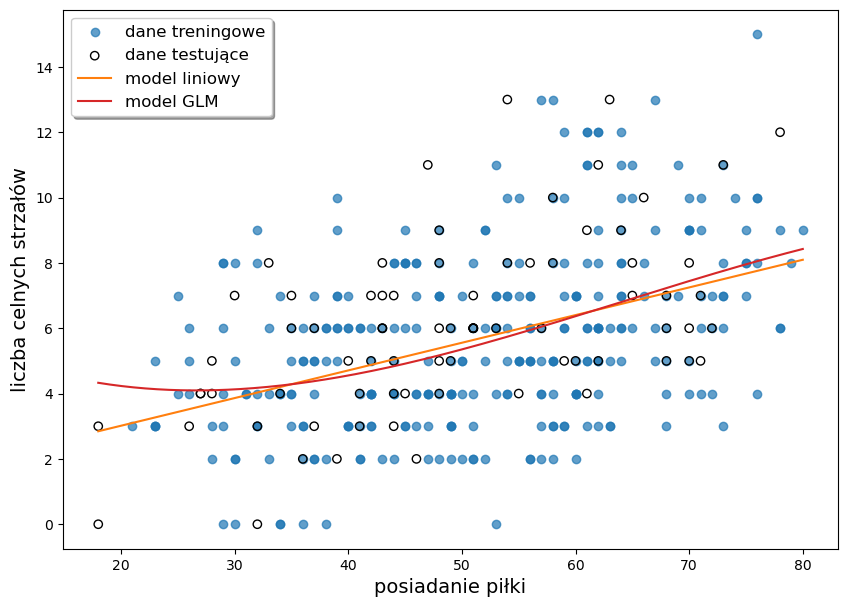
\includegraphics[scale=0.30]{shots_on_target.png}
    \caption{Posiadanie piłki, a liczba strzałów celnych}
    \end{figure}

     Regresja liniowa jest postaci:
    \begin{equation}
    y = 0.08468 + 1.32104
    \end{equation}

    Parametry wielomianu stopnia 3:

    \begin{center}
    \begin{tabular}{| c | c | c | c |}
    \hline
    a & b & c & d \\ \hline
    -0.2102 & 0.005 & 0 & 6.65021 \\ \hline
    \end{tabular}
    \end{center}

    Dane zostały podzielone na zbiór treningowy i testowy w proporcji 80:20.
    \newline
    \newline
    Błąd średniokwadratowy:
    \begin{itemize}
    \item Regresja liniowa: \newline
    - dane treningowe: 6.06 \newline
    - dane testowe: 5.34
    \item Model GLM: \newline
    - dane treningowe: 6.06 \newline
    - dane testowe: 5.61
    \end{itemize}

    Dane są rozrzucone po wykresie, więc błąd średniokwadratowy jest dość duży, Współczynnik regresji liniowej dodatni, tendencja jest wzrostowa.
    \newpage
    \item Eksperyment 2 \newline

    \begin{figure}[hbt]
    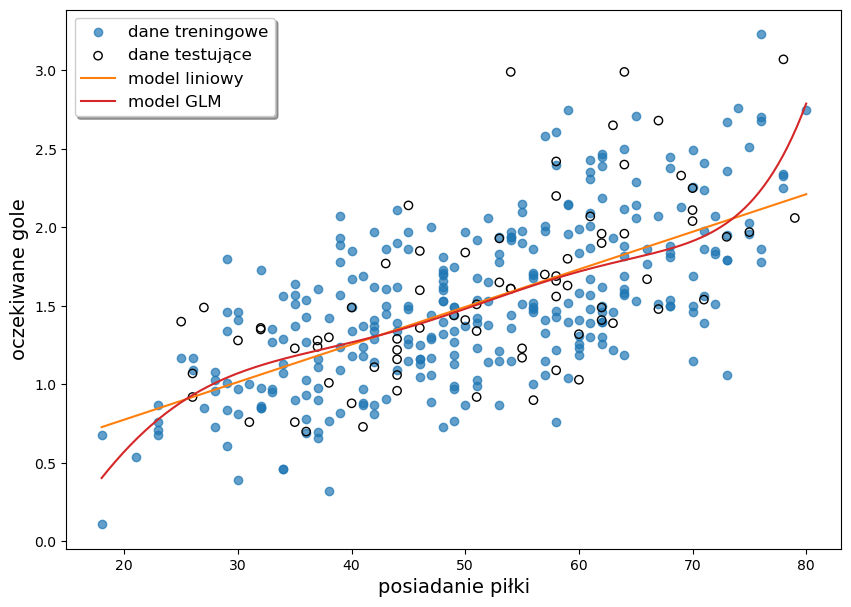
\includegraphics[scale=0.30]{xgoals.png}
    \caption{Posiadanie piłki w zależności od oczekiwanych goli}
    \end{figure}
    Regresja liniowa jest postaci:
    \begin{equation}
    y = 0.02377x + 0.32897
    \end{equation}

    Parametry wielomianu stopnia 3:
    \begin{center}
    \begin{tabular}{| c | c | c | c |}
    \hline
    a & b & c & d \\ \hline
    0.0908 & -0.0015 & 0 & -0.56232 \\ \hline
    \end{tabular}
    \end{center}
    
    Dane zostały podzielone na zbiór treningowy i testowy w proporcji 80:20.
    \newline
    \newline
    Błąd średniokwadratowy:
    \begin{itemize}
    \item Regresja liniowa: \newline
    - dane treningowe: 0.16 \newline
    - dane testowe: 0.15
    \item Model GLM: \newline
    - dane treningowe: 0.16 \newline
    - dane testowe: 0.149
    \end{itemize}
    
    Najlepiej dopasowanym wielomianem okazał się wielomian o stopniu 3. Dane są skupione, widać silną zależność między nimi, o czym świadczą małe wartości błędów średniokwadratowych dla danych treningowych oraz testowych. W tym kontekście należy wziąć też pod uwagę skale wartości oczekiwanych goli. Współczynnik regresji liniowej jest dodatni, tendencja danych jest wzrostowa.

    
    \item Eksperyment 3 \newline

    \begin{figure}[hbt]
    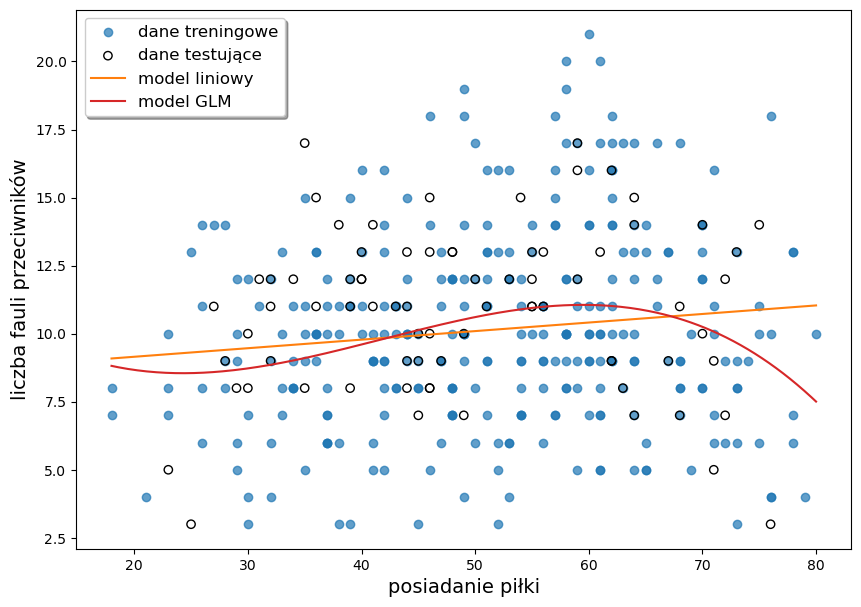
\includegraphics[scale=0.30]{fouls.png}
    \caption{Posiadanie piłki, a faule popełnione przez przeciwnika}
    \end{figure}

    Regresja liniowa jest postaci:
    \begin{equation}
    y = 0.03143x + 8.52269
    \end{equation}
    \newpage
      Parametry wielomianu stopnia 3:
    \begin{center}
    \begin{tabular}{| c | c | c | c |}
    \hline
    a & b & c & d \\ \hline
    -0.4992 & 0.0145 & -0.001 & 13.78565 \\ \hline
    \end{tabular}
    \end{center}
    
    Dane zostały podzielone na zbiór treningowy i testowy w proporcji 80:20.
    \newline
    \newline
     Błąd średniokwadratowy:
    \begin{itemize}
    \item Regresja liniowa: \newline
    - dane treningowe: 12.7 \newline
    - dane testowe: 9.39
    \item Model GLM: \newline
    - dane treningowe: 12.7 \newline
    - dane testowe: 8.85
    \end{itemize}

    Dane są bardzo rozrzucone, wysoki bład średniokwadratowy. Posiadanie piłki nie ma wiele wspólnego z liczbą fauli przeciwnika.
    
    \item Eksperyment 4 \newline

    \begin{figure}[hbt]
    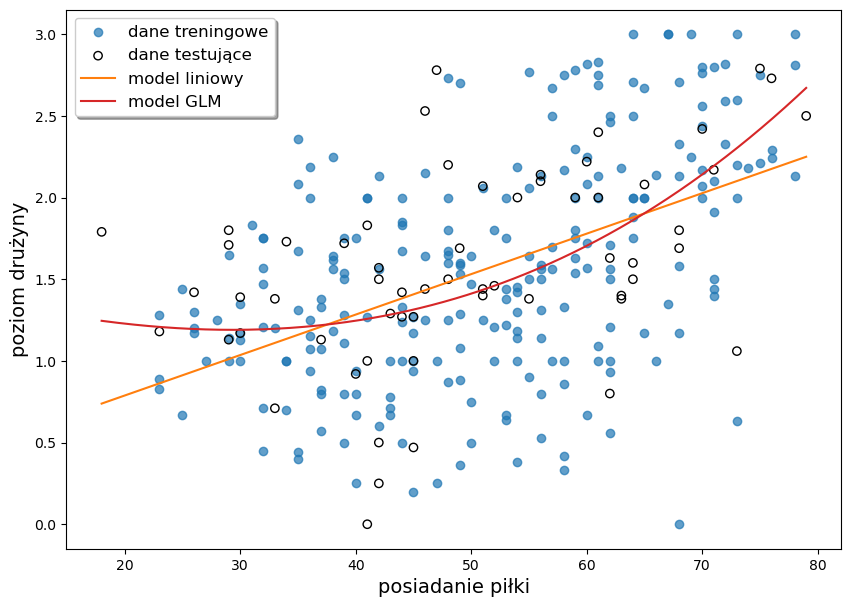
\includegraphics[scale=0.30]{level.png}
    \caption{Posiadanie piłki, a poziom drużyny(pkty/mecz)}
    \end{figure}

    Regresja liniowa jest postaci:
    \begin{equation}
    y = 0.02477x + 0.29257
    \end{equation}
    
      Parametry wielomianu stopnia 3:
    \begin{center}
    \begin{tabular}{| c | c | c | c |}
    \hline
    a & b & c & d \\ \hline
    -0.0198 & 0.0002 & 0 & 1.51629 \\ \hline
    \end{tabular}
    \end{center}

    Dane zostały podzielone na zbiór treningowy i testowy w proporcji 80:20.
    \newline
    \newline
    \newpage
     Błąd średniokwadratowy:
    \begin{itemize}
    \item Regresja liniowa: \newline
    - dane treningowe: 0.359 \newline
    - dane testowe: 0.296
    \item Model GLM: \newline
    - dane treningowe: 0.359 \newline
    - dane testowe: 0.276
    \end{itemize}

    
    Przed wykonaniem eksperymentu postanowiono odrzucić dane z pierwszych 8 kolejek, ponieważ średnia punktowa wtedy przyjmuje bardzo skrajne wartości, z każdą kolejką średnia lepiej się kształtowała.
    
    Zauważono wysoką zależność pomiędzy poziomem drużyny a posiadaniem piłki. Drużyny, które wysoko punktują, częsciej się utrzymują przy piłce i kreują sytuacje.
    
    \item Eksperyment 5 \newline

    \begin{figure}[hbt]
    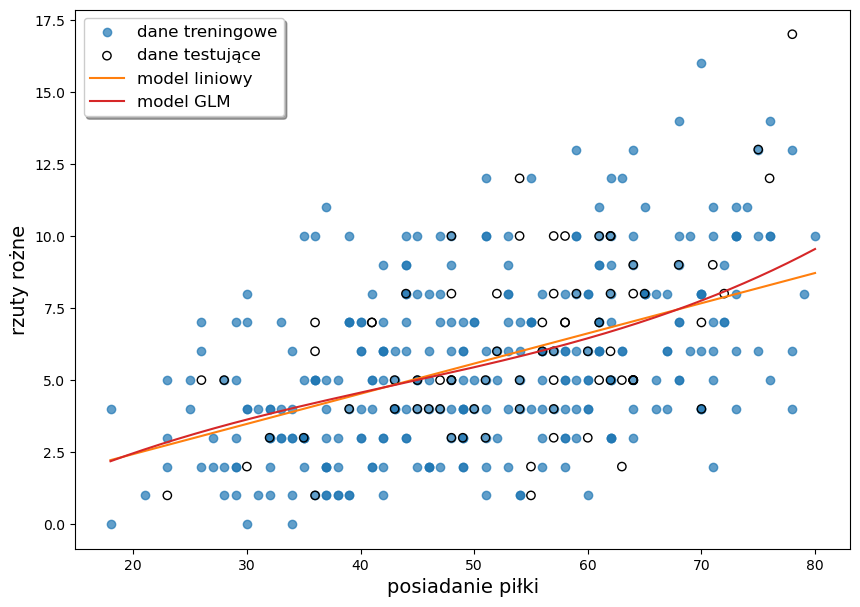
\includegraphics[scale=0.30]{corners.png}
    \caption{Posiadanie piłki, a rzuty rożne}
    \end{figure}

    Regresja liniowa jest postaci:
    \begin{equation}
    y = 0.1047 + 0.33929
    \end{equation}
    
    Parametry wielomianu stopnia 3:
    \begin{center}
    \begin{tabular}{| c | c | c | c |}
    \hline
    a & b & c & d \\ \hline
    0.2528 & -0.0039 & 0 & -1.29023 \\ \hline
    \end{tabular}
    \end{center}

    Dane zostały podzielone na zbiór treningowy i testowy w proporcji 80:20.
    \newline
    \newline
    Błąd średniokwadratowy:
    \begin{itemize}
    \item Regresja liniowa: \newline
    - dane treningowe: 6.97 \newline
    - dane testowe: 6.54
    \item Model GLM: \newline
    - dane treningowe: 6.97 \newline
    - dane testowe: 6.3
    \end{itemize}

    Najlepiej dopasowanym wielomianem okazał się
    wielomian 3. stopnia. Dane są jednak bardzo
    mocno rozrzucone, Wartości błędów średniokwadratowych
    dla danych treningowych oraz testowych są
    bardzo duże. Współczynnik regresji liniowej
    jest dodatni, tendencja danych jest wzrostowa.
    \item Eksperyment 6 \newline
    
    \begin{figure}[hbt]
    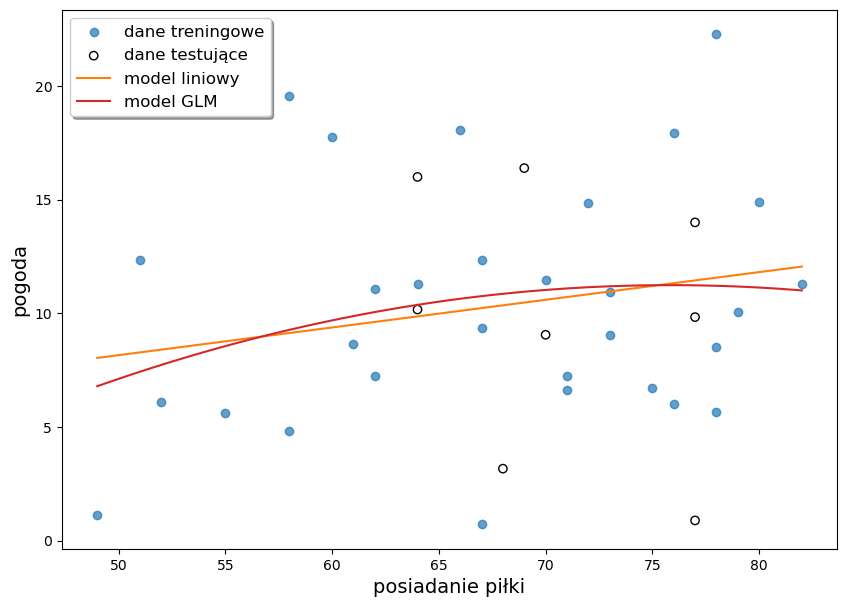
\includegraphics[scale=0.30]{weather.png}
    \caption{Posiadanie piłki Manchesteru City, a pogoda}
    \end{figure}

    Regresja liniowa jest postaci:
    \begin{equation}
    y = 0.12178 + 2.07017
    \end{equation}
    
    Parametry wielomianu stopnia 2:
    \begin{center}
    \begin{tabular}{| c | c | c |}
    \hline
    a & b & c \\ \hline
    0.9351 & -0.0062 & -24.2291 \\ \hline
    \end{tabular}
    \end{center}

    Dane zostały podzielone na zbiór treningowy i testowy w proporcji 80:20.
    \newline

    Błąd średniokwadratowy:
    \begin{itemize}
    \item Regresja liniowa: \newline
    - dane treningowe: 25.3 \newline
    - dane testowe: 30.9
    \item Model GLM: \newline
    - dane treningowe: 25.3 \newline
    - dane testowe: 30.1
    \end{itemize}
    
    Z obserwacji wynika, że posiadanie piłki w przypadku tej drużyny nie wynika w żadnym stopniu z warunków pogodowych. Dane są mocno rozrzucone po wykresie.
    
\end{enumerate}

\section{Modelowanie}

    Stworzony został model predykujący posiadanie piłki. Został wytrenowany na parametrach które wykazały większą zależność z posiadaniem piłki niż pozostałe. Był to współczynnik oczekiwanych goli, poziom drużyny i liczba strzałów celnych w meczu. Najlepszym modelem okazał się ten wykorzystujący regresję liniową. Jego współczynnik determinacji wynosi
    \begin{equation}
    R^2 = 0.58
    \end{equation}
    To sugeruje, że istnieje umiarkowana zależność między tymi czynnikami a posiadaniem piłki.
    
    
    \begin{figure}[hbt]
    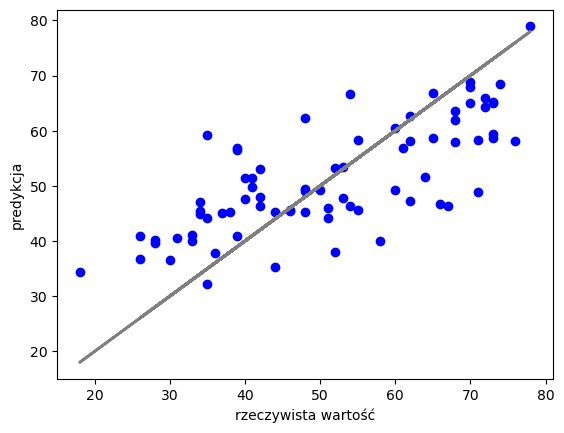
\includegraphics[scale=0.40]{predict_real.png}
    \caption{Rzeczywista wartość a wartość predykowana}
    \end{figure}
    Wykres porównuje rzeczywistą wartość ze zbioru testowego i wartość predykowaną. Jeśli punkt na wykresie znajduje się na prostej y=x, oznacza to że model przewidział dobrze wartość.
    \newline
    \newline
    Model jest w stanie w pewnym stopniu przewidywać, która drużyna będzie miała kontrolę nad piłką na podstawie tych zmiennych. Jednak pozostałe 42\% wariantów pozostaje niewyjaśnione przez model liniowy, co sugeruje, że istnieją inne czynniki, które również wpływają na posiadanie piłki i nie zostały uwzględnione w analizie.
    \newline
    \newline
    Dokonano jeszcze klasyfikacji zbioru na trzy klasy charakteryzujące posiadanie:
    \begin{itemize}
    \item \textbf{Niskie:} $\leq$38\%
    \item \textbf{Średnie:} 39\%-64\%
    \item \textbf{Wysokie:} $\geq$65\%
    \end{itemize}
    Wartości przedziałów zostały określone na podstawie mediany i odchylenia standardowego.
    Podziału dokonano używając regresji logistycznej.
    \begin{table}[hbt]
    \centering
    \begin{tabular}{lccc}
    \hline
    \textbf{Klasa} & \textbf{Precyzja} & \textbf{Czułość} & \textbf{Miara F1} \\
    \hline
    Wysokie   & 1.00 & 0.14 & 0.25 \\
    Średnie & 0.56 & 0.95 & 0.70 \\
    Niskie  & 0.80 & 0.44 & 0.57 \\
    \hline
    \textbf{Dokładność} &  &  & 0.61 \\
    \textbf{Średnia} & 0.79 & 0.51 & 0.51 \\
    \textbf{Ważona}  & 0.74 & 0.61 & 0.55 \\
    \hline
    \end{tabular}
    \caption{Wyniki klasyfikacji}
    \end{table}

    Model regresji logistycznej osiągnął dobre wyniki precyzji dla klas "Wysokie" i "Niskie", ale słabsze wyniki dla klasy "Średnie". Czułość była za to wysoka dla klasy "Średnie". Miary F1 dla klas "Średnie" i "Niskie" są dobre.
    \newline

     \begin{figure}[hbt]
    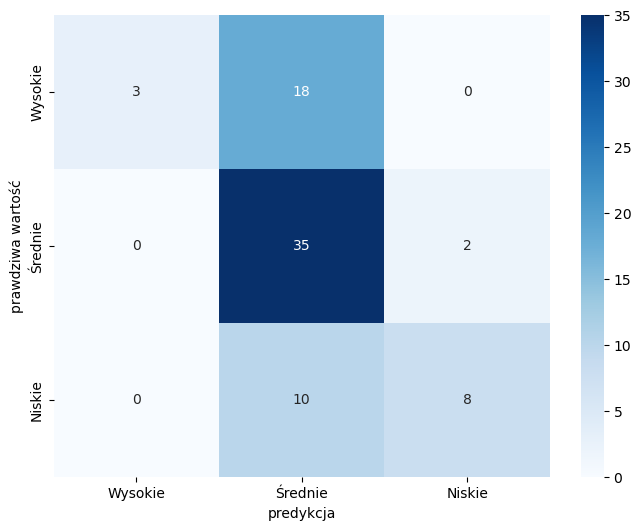
\includegraphics[scale=0.40]{confusions.png}
    \caption{Macierz pomyłek}
    \end{figure}
    Na macierzy pomyłek widać dobrze, że największa trudność zachodziła dla klasy "Średnie". \newline
    Model potrafi dobrze sklasyfikować 61\% obiektów. Wartości średniej i ważonej średniej wskazują, że ogólnie model ma równowagę, ale istnieje jeszcze pole do poprawy, szczególnie dla klasy "Wysokie".
    
\section{Wnioski}
%\renewcommand{\thesection}{\Roman{section}}

Po przeprowadzeniu eksperymentów należy stwierdzić, że posiadanie piłki nie zależy od liczby fauli przeciwnika, pogody, czy liczby rzutów rożnych. Statystyki te w meczu przyjmują różne wartości, jest w nich dużo losowości.

Zauważono jednak solidną zależność między posiadaniem piłk, a wskaźnikiem oczekiwanych goli, poziomem drużyny, czy też liczbą oddanych celnych strzałów. Te statystyki mówią, że drużyna stwarza sytuacje bramkowe, przeważa, a więc posiada też piłkę. Udało się więc stworzyć model estymujący posiadanie piłki drużyny na podstawie wybranych czynników, który radzi sobie umiarkowanie.
\newline
 Posiadanie piłki w meczu piłki nożnej może być wynikiem wielu czynników, również tych niemierzalnych lub ciężko mierzalnych takich jak taktyka drużyny, strategia przeciwników, zależność od wydarzeń boiskowych, kontuzji, zmęczenia, pewnej losowości.

\printbibliography[title={Bibliografia}]

\end{document}